% !TEX TS-program = XeLaTeX
% use the following command:
% all document files must be coded in UTF-8
\documentclass[spanish]{textolivre}
% build HTML with: make4ht -e build.lua -c textolivre.cfg -x -u article "fn-in,svg,pic-align"

\journalname{Texto Livre}
\thevolume{15}
%\thenumber{1} % old template
\theyear{2022}
\receiveddate{\DTMdisplaydate{2022}{6}{27}{-1}} % YYYY MM DD
\accepteddate{\DTMdisplaydate{2022}{7}{20}{-1}}
\publisheddate{\DTMdisplaydate{2022}{8}{23}{-1}}
\corrauthor{Ernesto Colomo Magaña}
\articledoi{10.35699/1983-3652.2022.40275}
%\articleid{NNNN} % if the article ID is not the last 5 numbers of its DOI, provide it using \articleid{} commmand 
% list of available sesscions in the journal: articles, dossier, reports, essays, reviews, interviews, editorial
\articlesessionname{articles}
\runningauthor{Gabarda Méndez et al.} 
%\editorname{Leonardo Araújo} % old template
\sectioneditorname{Hugo Heredia Ponce}
\layouteditorname{Carolina Garcia}

\title{El aprendizaje de las matemáticas mediante tecnología en Europa: revisión de literatura}
\othertitle{Aprendizagem de matemática aprimorada por tecnologia na Europa: uma revisão de literatura}
\othertitle{Technology-enhanced mathematics learning in Europe: a literature review}
% if there is a third language title, add here:
%\othertitle{Artikelvorlage zur Einreichung beim Texto Livre Journal}

\author[1]{Vicente Gabarda Méndez \orcid{0000-0001-6159-5173} \thanks{Email: \href{mailto:vicente.gabarda@uv.es}{vicente.gabarda@uv.es}}}
\author[2]{Ernesto Colomo Magaña \orcid{0000-0002-3527-7937} \thanks{Email: \href{mailto:ecolomo@uma.es}{ecolomo@uma.es}}}
\author[3]{Julio Ruiz Palmero \orcid{0000-0002-6958-0926} \thanks{Email: \href{mailto:julioruiz@uma.es}{julioruiz@uma.es}}}
\author[4]{Andrea Cívico Ariza  \orcid{0000-0003-3094-5841} \thanks{Email: \href{mailto:andrea.civico@campusviu.es}{andrea.civico@campusviu.es}}}
\affil[1]{Universitat de Valencia, Facultad de Filosofía y Ciencias de la Educación, Departamento de Didáctica y Organización Escolar, Valencia, España.}
\affil[2]{Universidad de Málaga, Facultad de Ciencias de la Educación, Departamento de Teoría e Historia de la Educación, Málaga, España.}
\affil[3]{Universidad de Málaga. Facultad de Ciencias de la Educación. Departamento de Didáctica y Organización Escolar, Málaga, España.}
\affil[4]{Universidad Internacional de Valencia, Facultad de Educación, Valencia, España.}

\addbibresource{article.bib}
% use biber instead of bibtex
% $ biber article

% used to create dummy text for the template file
\definecolor{dark-gray}{gray}{0.35} % color used to display dummy texts
\usepackage{lipsum}
\SetLipsumParListSurrounders{\colorlet{oldcolor}{.}\color{dark-gray}}{\color{oldcolor}}

% used here only to provide the XeLaTeX and BibTeX logos
\usepackage{hologo}

% if you use multirows in a table, include the multirow package
\usepackage{multirow}

% provides sidewaysfigure environment
\usepackage{rotating}

% CUSTOM EPIGRAPH - BEGIN 
%%% https://tex.stackexchange.com/questions/193178/specific-epigraph-style
\usepackage{epigraph}
\renewcommand\textflush{flushright}
\makeatletter
\newlength\epitextskip
\pretocmd{\@epitext}{\em}{}{}
\apptocmd{\@epitext}{\em}{}{}
\patchcmd{\epigraph}{\@epitext{#1}\\}{\@epitext{#1}\\[\epitextskip]}{}{}
\makeatother
\setlength\epigraphrule{0pt}
\setlength\epitextskip{0.5ex}
\setlength\epigraphwidth{.7\textwidth}
% CUSTOM EPIGRAPH - END

% LANGUAGE - BEGIN
% ARABIC
% for languages that use special fonts, you must provide the typeface that will be used
% \setotherlanguage{arabic}
% \newfontfamily\arabicfont[Script=Arabic]{Amiri}
% \newfontfamily\arabicfontsf[Script=Arabic]{Amiri}
% \newfontfamily\arabicfonttt[Script=Arabic]{Amiri}
%
% in the article, to add arabic text use: \textlang{arabic}{ ... }
%
% RUSSIAN
% for russian text we also need to define fonts with support for Cyrillic script
% \usepackage{fontspec}
% \setotherlanguage{russian}
% \newfontfamily\cyrillicfont{Times New Roman}
% \newfontfamily\cyrillicfontsf{Times New Roman}[Script=Cyrillic]
% \newfontfamily\cyrillicfonttt{Times New Roman}[Script=Cyrillic]
%
% in the text use \begin{russian} ... \end{russian}
% LANGUAGE - END

% EMOJIS - BEGIN
% to use emoticons in your manuscript
% https://stackoverflow.com/questions/190145/how-to-insert-emoticons-in-latex/57076064
% using font Symbola, which has full support
% the font may be downloaded at:
% https://dn-works.com/ufas/
% add to preamble:
% \newfontfamily\Symbola{Symbola}
% in the text use:
% {\Symbola }
% EMOJIS - END

% LABEL REFERENCE TO DESCRIPTIVE LIST - BEGIN
% reference itens in a descriptive list using their labels instead of numbers
% insert the code below in the preambule:
%\makeatletter
%\let\orgdescriptionlabel\descriptionlabel
%\renewcommand*{\descriptionlabel}[1]{%
%  \let\orglabel\label
%  \let\label\@gobble
%  \phantomsection
%  \edef\@currentlabel{#1\unskip}%
%  \let\label\orglabel
%  \orgdescriptionlabel{#1}%
%}
%\makeatother
%
% in your document, use as illustraded here:
%\begin{description}
%  \item[first\label{itm1}] this is only an example;
%  % ...  add more items
%\end{description}
% LABEL REFERENCE TO DESCRIPTIVE LIST - END


% add line numbers for submission
%\usepackage{lineno}
%\linenumbers

\newcolumntype{N}[1]{>{\raggedright\arraybackslash}p{#1}}

\begin{document}
\maketitle

\begin{polyabstract}
\begin{abstract}
La integración de la tecnología en los procesos formativos es una realidad en los diferentes sistemas educativos internacionales, estando presente de manera transversal o específica en el aprendizaje de las diferentes materias en las distintas etapas formativas. Este trabajo aborda específicamente el modo en que esta se utiliza como herramienta metodológica al servicio de la enseñanza y el aprendizaje de las matemáticas en la etapa de Educación Secundaria. Tomando como contexto geográfico la Unión Europea, se realiza una revisión sistemática de la literatura científica alojada en la base de datos de \textit{Web Of Science} de los últimos cinco años. Los resultados arrojan que la producción científica es prolífica, especialmente en los dos últimos años y en el contexto español; que las herramientas tecnológicas utilizadas son diversas; y que, independientemente de estas cuestiones, se concibe que estas tienen un impacto positivo en los procesos formativos de las matemáticas, tanto para los estudiantes como para los docentes.

\keywords{Matemáticas \sep Tecnologías \sep Educación secundaria \sep Unión Europea \sep Estudio bibliográfico}
\end{abstract}

\begin{portuguese}
\begin{abstract}
A integração da tecnologia nos processos formativos é uma realidade nos diferentes sistemas educativos internacionais, estando presente de forma transversal ou específica na aprendizagem das diferentes disciplinas nas diferentes etapas formativas. Este trabalho trata especificamente da forma como ela é utilizada como ferramenta metodológica a serviço do ensino e da aprendizagem da matemática no ensino médio. Tomando a União Europeia como contexto geográfico, é realizada uma revisão sistemática da literatura científica hospedada na base de dados Web Of Science dos últimos cinco anos. Os resultados mostram que a produção científica é prolífica, especialmente nos últimos dois anos e no contexto espanhol; que as ferramentas tecnológicas utilizadas são diversas; e que, independentemente dessas questões, se concebe que elas tenham um impacto positivo nos processos formativos da matemática, tanto para alunos quanto para professores.

\keywords{Matemática \sep Tecnologias \sep Educação secundária \sep União Europeia \sep Estudo bibliográfico}
\end{abstract}
\end{portuguese}

\begin{english}
\begin{abstract}
The integration of technology in educational processes is a reality in different international education systems, being included in a transversal or specific way in the learning of the different subjects in different educational stages. This paper deals  specifically addresses the way in which technology is used as a methodological tool in the teaching and learning of Mathematics at the Secondary Education in high school. Taking the European Union as a geographical context, a systematic review of the scientific literature hosted in the Web of Science database over the last five years is carried out. The results show that the scientific production is prolific, especially in the last two years and in the Spanish context; that the technological tools used are diverse; and that, regardless of these issues, they are considered to have a positive impact on the educational processes of Mathematics, for both students and teachers.

\keywords{Mathematics \sep Technologies \sep Secondary education  \sep European Union \sep Literature review}
\end{abstract}
\end{english}
% if there is another abstract, insert it here using the same scheme
\end{polyabstract}

\section{Introducción}

Los procesos formativos, en las últimas décadas, se han caracterizado por una integración progresiva de la tecnología en el diseño, el desarrollo y la evaluación de las acciones educativas de cualquier etapa.

Esta digitalización responde a múltiples motivaciones: por un lado, es importante que el ámbito educativo se desarrolle de manera alineada a otros ámbitos de la realidad (social, económico, productivo, etc.). Para ello, las diferentes políticas, tanto a nivel nacional como internacional, han tratado de promover la integración de la tecnología, tanto desde un punto de vista transversal en todas las etapas, como mediante contenidos específicos en algunas de ellas \cite{colomo__percepcion_2020}. Por otro lado, la utilización de la tecnología como herramienta metodológica se ha vinculado a un cambio de paradigma del propio hecho educativo, donde el estudiante se convierte en un eje fundamental del aprendizaje y se busca el modo de dotar al proceso formativo de una nueva mirada más cercana a sus intereses y necesidades, a la par que más innovadora. Esta realidad ha permitido no solamente el diseño de tecnologías \textit{ad hoc} para el contexto educativo, sino la adaptación de otras herramientas ajenas a él con fines formativos. Por último, no podemos obviar que la reciente situación de pandemia mundial derivada de la COVID-19 ha supuesto la puesta en marcha de procesos de hibridación o de modelos en línea que permitieran continuar con el aprendizaje desde casa \cite{cuevas__flipped_2020}.

Parece, además, que la tecnología y las matemáticas (área en la que se centra nuestro estudio) son áreas interconectadas, formando parte ambas de la metodología STEM (Science, Technology, Engineering \& Mathematics). Esta propuesta, no exenta de controversias en su definición e implementación \cite{bogdan_stem_2021}, se orienta hacia el aprendizaje de las disciplinas consideradas científicas, mediante métodos experienciales, para dar respuesta a las demandas de la sociedad actual \cite{acar_effects_2018}, siendo precisamente las matemáticas las que otorgan la base para el desarrollo del resto de ellas \cite{maass_role_2019}. De hecho, estudios como el de \textcite{diego-mantecon_steam_2021} ponen de manifiesto que las prácticas STEM contribuyen de forma inequívoca al desarrollo de la competencia matemática y de la competencia tecnológica.

Centrando el análisis en nuestra área de estudio, el desarrollo de destrezas matemáticas ha formado parte tradicionalmente de los currículos de toda etapa educativa y de cualquier contexto geográfico. La relevancia otorgada a esta área de conocimiento a nivel comunitario, más allá de su tradición histórica, encuentra su fundamento en el reconocimiento de la destreza matemática como una de las competencias clave para el aprendizaje permanente \cite{comision_recomendacion_2006,consejo_recomendacion_2018}. Contextualizada en relación con la competencia en ciencia, tecnología e ingeniería, la competencia matemática se vincula como la habilidad para desplegar y emplear el razonamiento matemático para la resolución de problemas en la vida cotidiana, materializándose específicamente en el cálculo, el pensamiento lógico y espacial, y la representación (fórmulas, gráficos, etc.).

Estas directrices comunitarias han servido para consolidar las matemáticas como área curricular en los diferentes sistemas educativos europeos, siendo una asignatura obligatoria en la práctica totalidad de los mismos, tanto en la etapa de Educación Primaria como en la de Educación Secundaria. De hecho, al margen de su presencia, es reseñable que representa la segunda mayor proporción de tiempo de instrucción (alrededor del 15\%-20\% del tiempo total de enseñanza) en la enseñanza obligatoria \cite{comision_recommended_2021}.

Además, cabe destacar que la integración de la tecnología en los procesos formativos en la Unión Europea constata que alrededor del 70\% de los estudiantes manifiestan utilizar Internet con fines educativos al menos una vez por semana \cite{comision_2nd_2019}, habiendo una diferencia considerable entre países como Dinamarca, donde la práctica totalidad lo hacen, o Eslovenia, donde solamente lo hace la mitad de ellos. En relación con los docentes, alrededor del 60\% utilizan la tecnología de forma habitual (en una cuarta parte o más de sus clases) a nivel europeo, siendo los profesores noruegos, daneses, malteses o lituanos quienes hacen un mayor uso de ella.

\section{La enseñanza y el aprendizaje de matemáticas mediante tecnología}

La tecnología ofrece unas posibilidades casi infinitas para la propuesta de actividades formativas mediadas por ella, bien sea mediante recursos digitales específicos, diseñados \textit{ad hoc}, como recursos metodológicos para un área en concreto o mediante tecnologías de carácter general que pueden ser implementadas como herramienta al servicio del proceso educativo.

La literatura científica previa avala que el uso de tecnología en la enseñanza y el aprendizaje de las matemáticas genera beneficios y mejoras en diferentes dimensiones, como en el rendimiento académico de los estudiantes \cite{martinez-garrido_impacto_2018}, así como para el aprendizaje significativo \cite{nivela__diseno_2018} o, de manera casi natural, para el desarrollo de las competencias matemática y digital \cite{valverde-crespo_competencia_2018}.

Si centramos nuestra atención en primer lugar en el uso de software especializado, destaca el uso de \textit{Geogebra}, presente en gran parte de la literatura científica. Esta herramienta contribuye a la mejora del rendimiento académico \cite{ardic_effect_2018}, haciéndola recomendable para el desarrollo de las destrezas matemáticas en cualquier etapa educativa \cite{alabdulaziz_effectiveness_2021}. En la misma línea apuntan los estudios de \textcite{birgin_effect_2020,munante-toledo_geogebra_2021,zulnaidi_effect_2019}, que han puesto de manifiesto el potencial específico de \textit{Geogebra} en el aprendizaje de las matemáticas, especialmente para una mejora del conocimiento conceptual y procedimental, y para la significatividad del aprendizaje y el rendimiento académico. Igualmente, \textcite{garcia_efectos_2021} concluyen que el uso de este \textit{software} aporta beneficios más allá de la esfera cognitiva, favoreciendo el desarrollo de relaciones afectivas entre los agentes. Además, cabe señalar que existe un impacto positivo de las aplicaciones móviles específicas para el aprendizaje de las matemáticas, evidenciado por estudios como el de \textcite{rodriguez-cubillo_uso_2021} o \textcite{alabdulaziz_covid-19_2021}, quienes, al margen de corroborar el aumento del rendimiento, resaltan el fomento de la motivación y la mejora de la actitud de los estudiantes hacia el área de conocimiento con el uso de la tecnología, junto con el desarrollo del pensamiento crítico.

Conjuntamente, tal y como apuntábamos anteriormente, se han venido implementado, en los últimos años, otro tipo de tecnologías que, sin estar creadas expresamente para los procesos de enseñanza y aprendizaje, han demostrado una serie de beneficios. Es el caso de la realidad aumentada, la cual favorece la comprensión de los conceptos, el desarrollo del pensamiento crítico y la autonomía, la motivación hacia el aprendizaje de las matemáticas y su individualización, así como el desarrollo de habilidades de investigación y la socialización entre estudiantes \cite{fernandez-enriquez_augmented_2020,kramarenko_prospects_2019} o el uso de foros virtuales \cite{juarez__interaccion_2020}, evaluando la incidencia de estas herramientas tanto en la interacción como en el nivel de profundidad desarrollado en el proceso de aprendizaje. Asimismo, otros estudios como el de \textcite{menjivar__revision_2021} ponen de relieve que la realidad virtual se utiliza de manera frecuente en el área de matemáticas, según la producción científica analizada.

También se ha demostrado el potencial de los videojuegos y la gamificación como recursos metodológicos para el aprendizaje de las matemáticas. De este modo, las propuestas de \textcite{kim_effects_2017,molina__resolucion_2020} o \textcite{pellas_systematic_2021}, advierten de los beneficios de estas herramientas para un aprendizaje más significativo, la resolución de problemas aritméticos y otras competencias transversales. Asimismo, existen propuestas donde la tecnología utilizada son simuladores \cite{diaz__aprendizaje_2018}, constatando su capacidad para la mejora del rendimiento académico o experiencias con blogs \cite{sanchez_uso_2016} o las tabletas \cite{guillen-gamez_digital_2018}, quienes subrayaban el potencial que tiene la tecnología para la organización y expresión del pensamiento matemático, facilitado por la portabilidad de algunas de las tecnologías.

La realidad que ponen de manifiesto estas experiencias, así como otras revisiones sistemáticas como las de \textcite{bano_mobile_2018}, junto con las políticas y directrices europeas, han servido de caldo de cultivo para el surgimiento de proyectos en el marco comunitario para la promoción del aprendizaje de las matemáticas mediante la tecnología. Algunos ejemplos de ello son el Proyecto MILAGE, que se orientaba a la integración de las tecnologías digitales en el área de matemáticas \cite{gonzales_integracion_2017}, o la plataforma \textit{STEMforYouth}, que integraba actividades en contextos reales para trabajar las matemáticas mediante metodologías como el aprendizaje mediante experimentación, el aprendizaje basado en investigación y la gamificación \cite{diego-mantecon_problemas_2018}.

A partir de este análisis, y con pretensión de comprender de forma más holística la utilización de la tecnología como herramienta metodológica para el aprendizaje de las matemáticas en Educación Secundaria, este estudio propone una revisión sistemática de la producción científica alojada en \textit{Web of Science} en los últimos cinco años sobre esta realidad.

\section{Metodología}

Este estudio se fundamenta en un análisis bibliográfico acerca de la literatura científica sobre la utilización de tecnología para la enseñanza y el aprendizaje de las matemáticas en Educación Secundaria en la Unión Europea.

Para realizar la búsqueda bibliográfica, se ha utilizado como base de datos \textit{Web of Science} (en adelante WOS), debido su potencial para dar cobertura a la literatura científica de ámbito internacional. Con relación a los términos de búsqueda, se han empleado “matemáticas”, “tecnología”, “aprendizaje” y “educación secundaria”, tanto en inglés como en español. La búsqueda devolvió un total de 123 resultados, los cuales han sido filtrados en base a los criterios de inclusión que se ofrecen a continuación:

\begin{table}[h!]
\centering
\begin{threeparttable}
\caption{Criterios de selección de documentos.}
\begin{tabular}{ll}
\toprule
Tipología & Artículos científicos \\
\midrule
Disponibilidad & Acceso abierto y texto completo \\
Tipo de estudio & Investigación empírica \\
Participantes & Profesorado o alumnado de educación secundaria \\
Fecha de publicación & 2017-2021 \\
Contexto geográfico & Unión Europea \\
Idioma & Cualquier lengua oficial de la Unión Europea \\
\bottomrule
\end{tabular}
\label{Tabla01}
\source{Elaboración propia.}
\end{threeparttable}
\end{table} 

Tras la selección de artículos, se realizó una búsqueda inversa, pero no se halló ninguna propuesta complementaria. Se muestra en la \cref{Figura01} todo el proceso de búsqueda y selección, fundamentado en el método PRISMA \cite{urrutia_declaracion_2010}:

\begin{figure}[htbp]
\centering
\caption{Proceso de selección de documentos.}
\begin{minipage}{.6\textwidth}
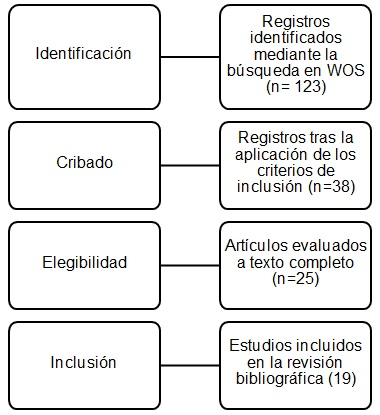
\includegraphics[width=\textwidth]{figura 01.jpg}
\label{Figura01}
\source{Elaboración propia.}
\end{minipage}
\end{figure}

Con los 19 documentos seleccionados, se realiza un análisis de contenido que se centrará en las siguientes variables de estudio:

\begin{table}[h!]
\centering
\begin{threeparttable}
\caption{Variables de análisis.}
\begin{tabular}{ll}
\toprule
Variables identificativas \\
\midrule
Fecha & Año de publicación  \\
País & Contexto geográfico de la investigación \\
Autoría & Relación de autores y coautores \\
Idioma & Lengua en que se publica el artículo \\
\toprule
Variables de contenido \\
\midrule
Muestra & Participantes del estudio \\
Diseño & Metodología implementada en el estudio \\
Objetivos & Fines que persigue el estudio \\
Tecnología & Herramienta digital utilizada \\
Resultados & Principales hallazgos del estudio \\
\bottomrule
\end{tabular}
\label{Tabla02}
\source{Elaboración propia.}
\end{threeparttable}
\end{table}

\section{Resultados}

En la \cref{Tabla03}, se recogen los datos de las 19 investigaciones objeto de estudio respecto a variables identificativas y de contenido:

\begingroup
\small 
\setlength\tabcolsep{2pt}
%\begin{threeparttable}
\begin{longtable}{*{2}{N{0.1\textwidth}}*{4}{N{0.19\textwidth}}}
\caption{Análisis de contenido.} 
\label{Tabla03}
\\
\toprule
Autor y año & País e idioma & Muestra y diseño & Objetivos & Tecnología & Resultados \\
\midrule
\arrayrulecolor[gray]{.7}
\textcite{del_cerro_application_2021} &
España \newline Inglés & 
48 estudiantes de Educación Secundaria Obligatoria \newline Cuasi\-expe\-rimen\-tal. Pretest-Postest & 
Averiguar si la integración del software \textit{Geogebra} AR (Realidad Aumentada) afecta al rendimiento académico y a las habilidades espaciales de los estudiantes. & Realidad Aumentada (\textit{Geogebra} AR) & 
La mayor parte de los estudiantes utiliza las TIC para estudiar matemáticas, aunque no consideran que les ayuden a mejorar sus notas. \\
\midrule
\textcite{hossein-mohand_uses_2021} &
España \newline Inglés &
2018 estudiantes de Educación Secundaria \newline
Cuasi\-expe\-rimen\-tal.
Pretest-Postest &
Analizar los factores que podrían influir en el uso de las TIC con fines educativos y determinar la variación del uso de las TIC con fines académicos (matemáticas) a raíz del COVID-19. &
Tecnología en general (sin especificar herramienta/s) &
El acceso a las TIC para fines educativos influye sobre el rendimiento en matemáticas \\
\midrule
\textcite{weinhandl_real-world_2021} &
Austria \newline Inglés &
Estudiantes y profesores de Educación Secundaria \newline
Estudio de caso. Cualitativo &
Explorar la influencia de la modelización matemática, utilizando la tecnología, sobre la adquisición de conocimientos y competencias matemáticas y sobre la creatividad. &
\textit{Geogebra} &
La aplicación de la modelización matemática apoyada en la tecnología favorece el intercambio de conocimientos tecnológicos y las competencias de los alumnos, así como sus conocimientos y competencias matemáticas. \\
\midrule
\textcite{weinhandl_look_2021} &
Austria \newline Inglés &
42 estudiantes y profesores de Educación Secundaria \newline
Estudio de caso. Cualitativo interpretativo &
Descubrir algunos elementos clave del éxito del aprendizaje de las  matemáticas en casa a raíz del COVID-19. & \textit{Geogebra} &
La utilización de la tecnología se constata como un elemento crucial para la transición de la enseñanza presencial a la educación en casa. Facilita, tanto la comunicación entre docente-discente, como con los compañeros, contribuyendo a la mejora de la colaboración y la estructura social del grupo. \newline
Además, favorece el trabajo autónomo y a la autorregulación del aprendizaje. \\
\midrule
\textcite{silva-diaz_uso_2021} &
España \newline Español &
17 estudiantes y un profesor de Educación Secundaria
Mixto. Pre-test-postest & 
Determinar el impacto de la Realidad Virtual Inmersiva en el desarrollo de actividades manipulativas y experienciales y sobre las actitudes científico-matemáticas de los alumnos. & Realidad Virtual Inmersiva & Los resultados indican que esta tecnología influye en la actitud hacia el aprendizaje de las matemáticas, así como en la autopercepción del aprendizaje. \\
\midrule
\textcite{petrov_effect_2020} & 
Bulgaria \newline Inglés &
Estudio de caso. \newline Estudio de caso. Pre-test-postest & 
Analizar el efecto de la realidad aumentada (RA) en el aprendizaje de las matemáticas. & Realidad Aumentada & El estudio ha demostrado una mejora en la comprensión de la materia estudiada, así como la significatividad del aprendizaje.
Se constata un mayor interés del estudiantado en el proceso formativo, así como su motivación. Favorece, asimismo, el trabajo cooperativo. \\
\midrule
\textcite{iglesias_aprendizaje_2020} &
España \newline Español &
27 estudiantes. \newline Descriptivo. & 
Analizar el impacto de la tecnología en la transición a la docencia no presencial por le COVID-19, especialmente, sobre el aprendizaje autónomo y la comunicación profesor-alumno. & 
Tecnología en general (sin especificar herramienta/s) &
Los resultados muestran que los alumnos superaron los criterios de evaluación de este bloque de contenidos y que se alcanzaron niveles óptimos de retroalimentación durante todo el proceso de enseñanza y aprendizaje. \\
\midrule
\textcite{gomez-garcia_technological_2020} &
España \newline Inglés &
2018 estudiantes. \newline Correlacional y pre-dictivo. &
Determinar las relaciones entre el rendimiento académico, los usos y los recursos TIC disponibles en el área de matemáticas. &
Tecnología en general (sin especificar herramienta/s) &
La mayor parte de los alumnos afirma que utiliza las TIC en casa para estudiar matemáticas.
El nivel educativo es un predictor del rendimiento académico en matemáticas asociado a los usos de las TIC por parte de los estudiantes. \\
\midrule
\textcite{gil-quintana_learning_2020} & 
Italia \newline Inglés &
4845 estudiantes. \newline Mixto. Descriptivo-correlacional. &
Diagnosticar el papel de la cultura participativa, los recursos digitales, las redes sociales y, en concreto, YouTube, en los procesos de aprendizaje y la adquisición de las competencias de Ciencia, Tecnología, Ingeniería y Matemáticas (STEM). & \textit{Youtube} &
Los adolescentes valoran los vídeos de YouTube como un recurso clave para mejorar su rendimiento escolar, valorando mejor a los \textit{youtubers} que a los profesores. Sin embargo, llama la atención que en los procesos de aprendizaje y adquisición de competencias STEM, prefieren interactuar con profesores antes que con \textit{youtubers}. \\
\midrule
\textcite{nunes_fatores_2020} &
Portugal \newline Portugués &
96 profesores. \newline Cuantitativo. Descriptivo y exploratorio. &
Explorar y describir los factores fundamentales que influyen en el conocimiento y uso de las (TIC), en particular del Software Educativo (SE) como herramienta, por parte de los profesores de matemáticas. &
\textit{Kahoot, Modellus y Scratch} & Los resultados sugieren que hay un conocimiento y uso escaso de estos recursos por parte del profesorado, constituyendo la edad, el género y la antigüedad de los profesores de matemáticas algunos factores que influyen en ello. \\
\midrule
\textcite{jesionkowska_active_2020} &
Reino Unido \newline Inglés &
Estudiantes y profesores. \newline Estudio de caso. Cualitativo interpretativo. & 
Analizar los beneficios del Aprendizaje Activo para la enseñanza de asignaturas STEAM, utilizando un software de realidad aumentada. &
Realidad Aumentada & Los estudiantes fueron capaces de crear aplicaciones funcionales y consideraron que la realidad aumentada mejoró su experiencia de aprendizaje. \\
\midrule
\textcite{jimenez_digital_2020} &
España \newline Inglés &
101 estudiantes. \newline Cuantiativo. Correlacional. & 
Estudiar el impacto del \textit{escape room digital}, utilizando \textit{Genial.ly} y un \textit{breakout}, para el aprendizaje del álgebra en el tercer curso de la educación secundaria para el aprendizaje de fracciones algebraicas y ecuaciones. & 
\textit{Escape room digital}, \textit{Genial.ly} y \textit{breakout} & Los resultados muestran que hay diferencias en relación con el aprendizaje de ecuaciones, concluyéndose que el uso de estas técnicas contribuye a la mejora de las calificaciones. Asimismo, los estudiantes tienen una percepción positiva de la experiencia, por la mejora de sus conocimientos, el aumento de la motivación y la promoción del trabajo en equipo. \\
\midrule
\textcite{curto__student_2019} &
España \newline Inglés &
68 estudiantes. \newline Pre-experimental. & Evaluar el uso de la aplicación \textit{Kahoot} en las asignaturas de matemáticas, biología y geología, y física y química. & \textit{Kahoot} & Los resultados apuntan que, en el área de matemáticas, esta herramienta tiene potencial para la autoevaluación, auto-nomía y autorregulación del proceso de aprendizaje, así como para la mejora de los resultados académicos. Asimismo, los estudiantes perciben que el aprendizaje es más divertido, activo y experiencial, favoreciendo la creatividad y aumentando la motivación. \\
\midrule
\textcite{lopez_formative_2019} &
España \newline Inglés & 
60 estudiantes. \newline Experimental. Descrip-tivo y correlacional (dos grupos). & Analizar la efectividad del \textit{flipped learning} sobre un enfoque tradicional de enseñanza y aprendizaje en la asignatura. & \textit{Flipped learning} & Los resultados reflejan que el \textit{flipped learning }mejora los indicadores y conocimientos matemáticos establecidos. Se concluye, además, que su uso incrementa la motivación y las habilidades en el análisis y representación de gráficos. \\
\midrule
\textcite{benitez__effects_2019} & 
España \newline Español &
1376 estudiantes. \newline Experimental. Correlacional entre grupos. & Evaluar el grado de asociación que el uso de las TIC podría tener con el rendimiento escolar en matemáticas. & Tecnología en general (sin especificar herramienta/s) & Los resultados reflejaron cambios positivos en el rendimiento escolar influidos por el uso eficaz de las TIC. Se demostró que el aprendizaje puede mejorarse gracias a las TIC, a menos que su uso no sea el adecuado. \\
\midrule
\textcite{aris_educational_2019} &
España \newline Inglés &
Estudiantes y profesores. \newline Pre-experimental. Descriptivo. & Analizar el impacto de la robótica educa-tiva (RE) sobre su impacto en el proceso de aprendizaje. & Robótica & Los resultados obtenidos permiten concluir que tanto profesores como alumnos consideran que este proyecto fomenta el interés y la curiosidad científica, así como las habilidades sociales a través del trabajo en equipo. \\
\midrule
\textcite{garcia-martin_use_2019} & 
España \newline Español & 
1488 estudiantes. \newline Cuantiativo. Correlacional. & Analizar el uso que hacen los adolescentes de cinco herramientas (buscadores, wikis, blogs, podcasts y mensajería instantánea), y el impacto que el uso de estas herramientas tiene en su rendimiento académico en ciencias, matemáticas, lengua española e inglés. & Buscadores, wikis, blogs, podcast y mensajería instantánea & Los participantes utilizaron los buscadores y los wikis para realizar tareas académicas y los podcasts para entretenerse. Las mujeres obtuvieron un mejor rendimiento en las áreas lingüísticas y los hombres en las científicas. El uso de buscadores se asoció a un mejor rendimiento en ciencias, lengua española e inglés, mientras que el uso de podcasts se asoció a un mejor rendimiento en matemáticas. \\
\midrule
\textcite{altanis_systematic_2018} &
Grecia \newline Inglés &
22 estudiantes. \newline Mixto. Descriptivo. & Analizar el efecto de la creación de jue-gos basados en el movimiento mediante la tecnología. & Cámaras & Los resultados indican que este enfoque puede aumentar la motivación de los estudiantes, reforzar su pensamiento computacional, mejorar su comprensión de los principios geométricos y mejorar sus habilidades sociales. \\
\midrule
\textcite{beltran_modelado_2017} & 
España \newline Español & 
15 alumnos. \newline Cualitativo. Interpretativo. & Analizar el uso de impresoras 3D en la enseñanza de las matemáticas. & Impresoras 3D & El modelado y la impresión 3D contribuyen a la comprensión de los contenidos curriculares vinculados con los objetos y sus significados.
\\
\arrayrulecolor{black}
\bottomrule
\source{Elaboración propia.}
\end{longtable}
\endgroup
%\end{threeparttable}

Atendiendo en primer lugar a las variables identificativas, es reseñable que, partiendo del rango de los últimos cinco años, la producción científica parece ir creciendo de manera progresiva. De este modo, hay un solo artículo de 2017 y de 2018, mientras que en el año 2020 hay 7 propuestas y, en el 2021, 5.

Por otro lado, la mayor parte de las investigaciones, dentro del ámbito comunitario, se contextualizan en España (12 de las 19 publicaciones), habiendo presencia de dos propuestas de Austria, mientras que con un estudio están países como Bulgaria, Italia, Portugal, Reino Unido y Grecia. Sin embargo, independientemente del contexto geográfico, la mayor parte de las publicaciones se realizan en lengua inglesa (13 de ellas), cinco en español y una en lengua portuguesa, respondiendo a las normas de publicación específicas de las revistas donde se publican.

Por último, en el caso de la autoría, es destacable que todos se realizan en coautoría (entre dos y cinco autores). Además, aunque con diferentes combinaciones, hay autores que están presentes en más de una propuesta, en cada uno de los dos contextos geográficos más habituales de las propuestas. De este modo, autores como Aris, Gómez-García, Hossein-Mohand, Hossein-Mohand, Orcos y Trujillo-Torres son autores de dos propuestas en el ámbito español (tres en el caso de Orcos), y Weinhandl y Lavicza comparten dos publicaciones en el contexto austríaco.

Si centramos la atención en el análisis del contenido de los artículos, la mayor parte de ellos toman como muestra a los estudiantes de Educación Secundaria, habiendo igualmente varios casos donde los participantes son tanto éstos mismos como los docentes que imparten matemáticas. De este modo, se trata de obtener una perspectiva global y complementaria entre los diferentes agentes que participan en el proceso formativo. En relación con el tamaño de la muestra, hay bastante variabilidad, pudiendo encontrar desde un estudio de caso \cite{petrov_effect_2020}, hasta estudios donde hay más de un millar de participantes, como los de \textcite{benitez__effects_2019,garcia-martin_use_2019,gomez-garcia_technological_2020,hossein-mohand_uses_2021}, llegando a más de cinco mil en el caso de \textcite{gil-quintana_learning_2020}. Por otro lado, respecto al diseño de investigación utilizado, encontramos diversidad de enfoques, aunque predominan las aproximaciones cuantitativas. De este modo, encontramos diseños de pretest y postest \cite{del_cerro_application_2021,hossein-mohand_uses_2021,petrov_effect_2020,silva-diaz_uso_2021} que analizan la mejora de la competencia matemática tras la aplicación de la tecnología en el proceso, otros estudios que plantean análisis entre grupos \cite{benitez__effects_2019,lopez_formative_2019}, otros de carácter correlacional, que abordan el impacto de otras variables en el aprendizaje, como los de \textcite{gil-quintana_learning_2020} o \textcite{gomez-garcia_technological_2020} y algunos de corte descriptivo como los de \textcite{aris_educational_2019} o \textcite{iglesias_aprendizaje_2020}. En la aproximación más cualitativa, se encuentran estudios como los de \textcite{beltran_modelado_2017} o \textcite{weinhandl_real-world_2021}, que les dotan de un abordaje centrado en la interpretación.

Los objetivos de las investigaciones se orientan principalmente hacia la comprobación del uso de tecnología para el aprendizaje de las matemáticas en general (si se utiliza algún tipo de herramienta digital para el desarrollo de destrezas matemáticas) o, las más comunes, hacia el análisis del impacto de alguna tecnología específica en el aprendizaje de las matemáticas. En el primer grupo (aquellas propuestas que estudian el uso o no de tecnologías), podemos encontrar los estudios de \textcite{hossein-mohand_uses_2021} o \textcite{iglesias_aprendizaje_2020}, quienes analizan los cambios metodológicos asociados a las acciones formativas a raíz de la COVID-19, en términos de comunicación docente-discente y de uso de las TIC en los procesos de aprendizaje. También analizan la utilización genérica de la tecnología en el aprendizaje de las matemáticas \textcite{gomez-garcia_technological_2020,benitez__effects_2019}, constatando que se usan herramientas digitales por parte de los estudiantes o, en el caso contrario, confirmando su falta de conocimiento y uso por parte de los docentes \cite{nunes_fatores_2020}. Por otro lado, como apuntábamos anteriormente, son más numerosas las propuestas que evalúan el impacto de tecnologías específicas en las acciones formativas. En esta categoría, podemos igualmente distinguir dos tipos de estudios: los que se centran en el uso de software especializado en el desarrollo de competencias matemáticas o científicas, y los que analizan el impacto de otro tipo de tecnología. En el caso de los primeros, hay un especial interés por conocer la utilidad de \textit{Geogebra} como herramienta metodológica \cite{del_cerro_application_2021,weinhandl_real-world_2021,weinhandl_look_2021}. También es destacable, por la naturaleza de la tecnología utilizada, que haya tres artículos vinculados al uso de la realidad aumentada \cite{jesionkowska_active_2020,petrov_effect_2020} y la realidad virtual inmersiva \cite{silva-diaz_uso_2021}, así como uno asociado al uso de impresoras 3D \cite{beltran_modelado_2017}, otro que se vincula al uso de \textit{Modellus} \cite{nunes_fatores_2020} y otro sustentado en el uso de la robótica \cite{aris_educational_2019}. En el último subgrupo de investigaciones, tendríamos aquellas que utilizan tecnología no especializada para el aprendizaje de las matemáticas. Este sería el caso de \textcite{gil-quintana_learning_2020}, quienes sustentan su estudio en el uso de \textit{Youtube}; \textcite{curto__student_2019}, que evalúan el uso de \textit{Kahoot}; \textcite{lopez_formative_2019}, con la implementación de una metodología \textit{flipped learning}; o \textcite{altanis_systematic_2018}, quienes evalúan el impacto del uso de cámaras. También estarían en este grupo las investigaciones de \textcite{jimenez_digital_2020}, quienes utilizan diferentes metodologías (\textit{escape room},\textit{Genial.ly} y \textit{breakout}) y \textcite{garcia-martin_use_2019}, que utilizan en su estudio buscadores, wikis, blogs, podcast y mensajería instantánea.

Por último, con relación a los resultados, pueden agruparse en dos grandes bloques: los relativos al rendimiento académico, y los que se asocian a otras cuestiones educativas. En el caso del impacto de la utilización de tecnología en el rendimiento académico en el área de matemáticas, aunque uno de los estudios no evidencia correlación entre ambas cuestiones \cite{del_cerro_application_2021}, se constata de manera generalizada que las calificaciones de los estudiantes mejoran con su uso \cite{benitez__effects_2019,gil-quintana_learning_2020,garcia-martin_use_2019,gomez-garcia_technological_2020,hossein-mohand_uses_2021}. Parece haber consenso, igualmente, en que la utilización de la tecnología como herramienta metodológica favorece la comprensión de los contenidos curriculares asociados a esta área \cite{beltran_modelado_2017,jesionkowska_active_2020,jimenez_digital_2020,petrov_effect_2020}. Por último, los resultados constatan que la integración de medios digitales en el área de matemáticas favorece el desarrollo de otras competencias, como el trabajo individual, la autonomía y la autorregulación \cite{curto__student_2019,weinhandl_look_2021} o las habilidades sociales y el trabajo cooperativo \cite{altanis_systematic_2018,iglesias_aprendizaje_2020,weinhandl_real-world_2021}, favoreciendo del mismo modo la mejora de la motivación de los estudiantes frente a los procesos formativos \cite{aris_educational_2019,lopez_formative_2019,silva-diaz_uso_2021}.

\section{Conclusiones}

La revisión sistemática de la literatura ha permitido identificar que, en los últimos cinco años, ha habido una producción científica reseñable sobre la utilización de tecnologías en la enseñanza y aprendizaje de las matemáticas en Educación Secundaria, una tendencia al alza ya confirmada por estudios como el de \textcite{hillmayr_potential_2020}. Este aumento de la producción científica responde no solamente a la innegable digitalización progresiva de los procesos formativos, sino a la situación derivada de la COVID-19, que ha supuesto la exploración de nuevos escenarios de aprendizaje desde los que diseñar, implementar y evaluar los procesos formativos desde el hogar. Aunque nuestro estudio se contextualiza en la Unión Europea por el alcance del proyecto al que se adscribe, la implementación de tecnología como respuesta a la pandemia en el área de matemáticas puede constatarse en estudios en otros contextos geográficos como Arabia Saudí \cite{alabdulaziz_covid-19_2021}, Franja de Gaza \cite{marban_primary_2021}, Singapur \cite{tay_implementation_2021} o Australia \cite{attard_exploration_2020}. Sería interesante, bajo esta perspectiva, poder analizar la tendencia durante los próximos años, a fin de poder vincular de manera más directa, la relación entre la pandemia y la producción científica en esta área.

Por otro lado, es reseñable que no se constata una correlación entre el país donde se evidencia una mayor producción científica (España) y los países donde, a tenor de los informes de la \textcite{comision_2nd_2019}, se hace un mayor uso de la tecnología con fines formativos en Educación Secundaria (Dinamarca, Malta o Lituania entre otros).

Con relación al contenido de las propuestas analizadas, se concluye que se utilizan herramientas digitales de carácter diverso. Cuando se trata de software específico para el área matemática destaca \textit{Geogebra}, en línea con las investigaciones previas \cite{alabdulaziz_effectiveness_2021}. No obstante, hay múltiples posibilidades para poder desarrollar las destrezas digitales mediante otros recursos como repositorios de vídeos, herramientas de evaluación o juegos en línea, poniendo de relieve la diversidad de opciones mediadas por tecnología para favorecer el aprendizaje de las matemáticas \cite{lino__revision_2022}.

No obstante, es evidente que la utilización de la tecnología para la enseñanza y el aprendizaje de las matemáticas, a tenor de los resultados, contribuye a la mejora del proceso formativo. De este modo, se ha constatado su potencial para el rendimiento académico \cite{ardic_effect_2018,martinez-garrido_impacto_2018,zulnaidi_effect_2019}, el aprendizaje significativo \cite{birgin_effect_2020,molina__resolucion_2020,nivela__diseno_2018} y la motivación de los estudiantes \cite{fernandez-enriquez_augmented_2020,kramarenko_prospects_2019,rodriguez-cubillo_uso_2021}.

A pesar del consenso que denota la revisión realizada, sería interesante seguir desarrollando esta línea de trabajo mediante el análisis de este mismo fenómeno en otras etapas educativas, como la educación primaria, así como ampliar el estudio más allá de la Unión Europea para conocer la realidad en otros contextos geográficos. Por último, consideramos que sería relevante analizar cuál es el papel que juegan aspectos como la formación del profesorado o la competencia digital docente \cite{guillen-gamez_analysis_2021a,guillen-gamez_examining_2021b,linde-valenzuela_digital_2022} en la implementación de experiencias mediadas por tecnología para el aprendizaje de las matemáticas. De este modo, se podrían conocer algunas de las limitaciones que condicionan la puesta en marcha de este tipo de estrategias y desarrollar propuestas institucionales que favorecieran la incorporación de estas herramientas en los procesos de enseñanza y aprendizaje de las matemáticas.

\section{Agradecimientos}

Este artículo forma parte del Proyecto Erasmus + IMAS (Increasing Mathematical Attainment in Schools), con referencia 2019-1-ES01-KA201-065104 (2019-2022), financiado por la Unión Europea.

\printbibliography\label{sec-bib}
% if the text is not in Portuguese, it might be necessary to use the code below instead to print the correct ABNT abbreviations [s.n.], [s.l.]
%\begin{portuguese}
%\printbibliography[title={Bibliography}]
%\end{portuguese}


%full list: conceptualization,datacuration,formalanalysis,funding,investigation,methodology,projadm,resources,software,supervision,validation,visualization,writing,review
\begin{contributors}[sec-contributors]
\authorcontribution{Vicente Gabarda Méndez}[conceptualization, formal analysis, methodology, resources, writing]
\authorcontribution{Ernesto Colomo Magaña}[conceptualization, validation, writing, review]
\authorcontribution{Julio Ruiz Palmero}[funding, projadm, supervision]
\authorcontribution{Andrea Cívico Ariza}[conceptualization, datacuration, investigation, writing]
\end{contributors}

\end{document}